% Results of the measured-motor-speed experiment for the A1 poster: simulation
% (3 training seeds per variant) and real flights (4 missions per policy).
% Generated by make_results_fig.py from the training outputs and logs/.
% Compile on its own, then: \includegraphics[width=\linewidth]{images/fig_rpm_results_poster.pdf}
\documentclass[12pt, border=6pt]{standalone}
\usepackage{pgfplots}
\usepgfplotslibrary{groupplots}
\pgfplotsset{compat=1.18}
\usetikzlibrary{calc}
\renewcommand{\familydefault}{\sfdefault}

\definecolor{ink}{RGB}{27,67,32}     % poster text green
\definecolor{cI}{HTML}{5090CD}       % I1 / A: 32-step action history, no motor speeds (149 inputs)
\definecolor{cC}{HTML}{E06A12}       % C: motor speeds + 4-step history (41)
\definecolor{cE}{HTML}{B0083F}       % E: motor speeds, no history (25)
\colorlet{cD}{black!45}              % D: 4-step history, no motor speeds (37), control

\begin{document}
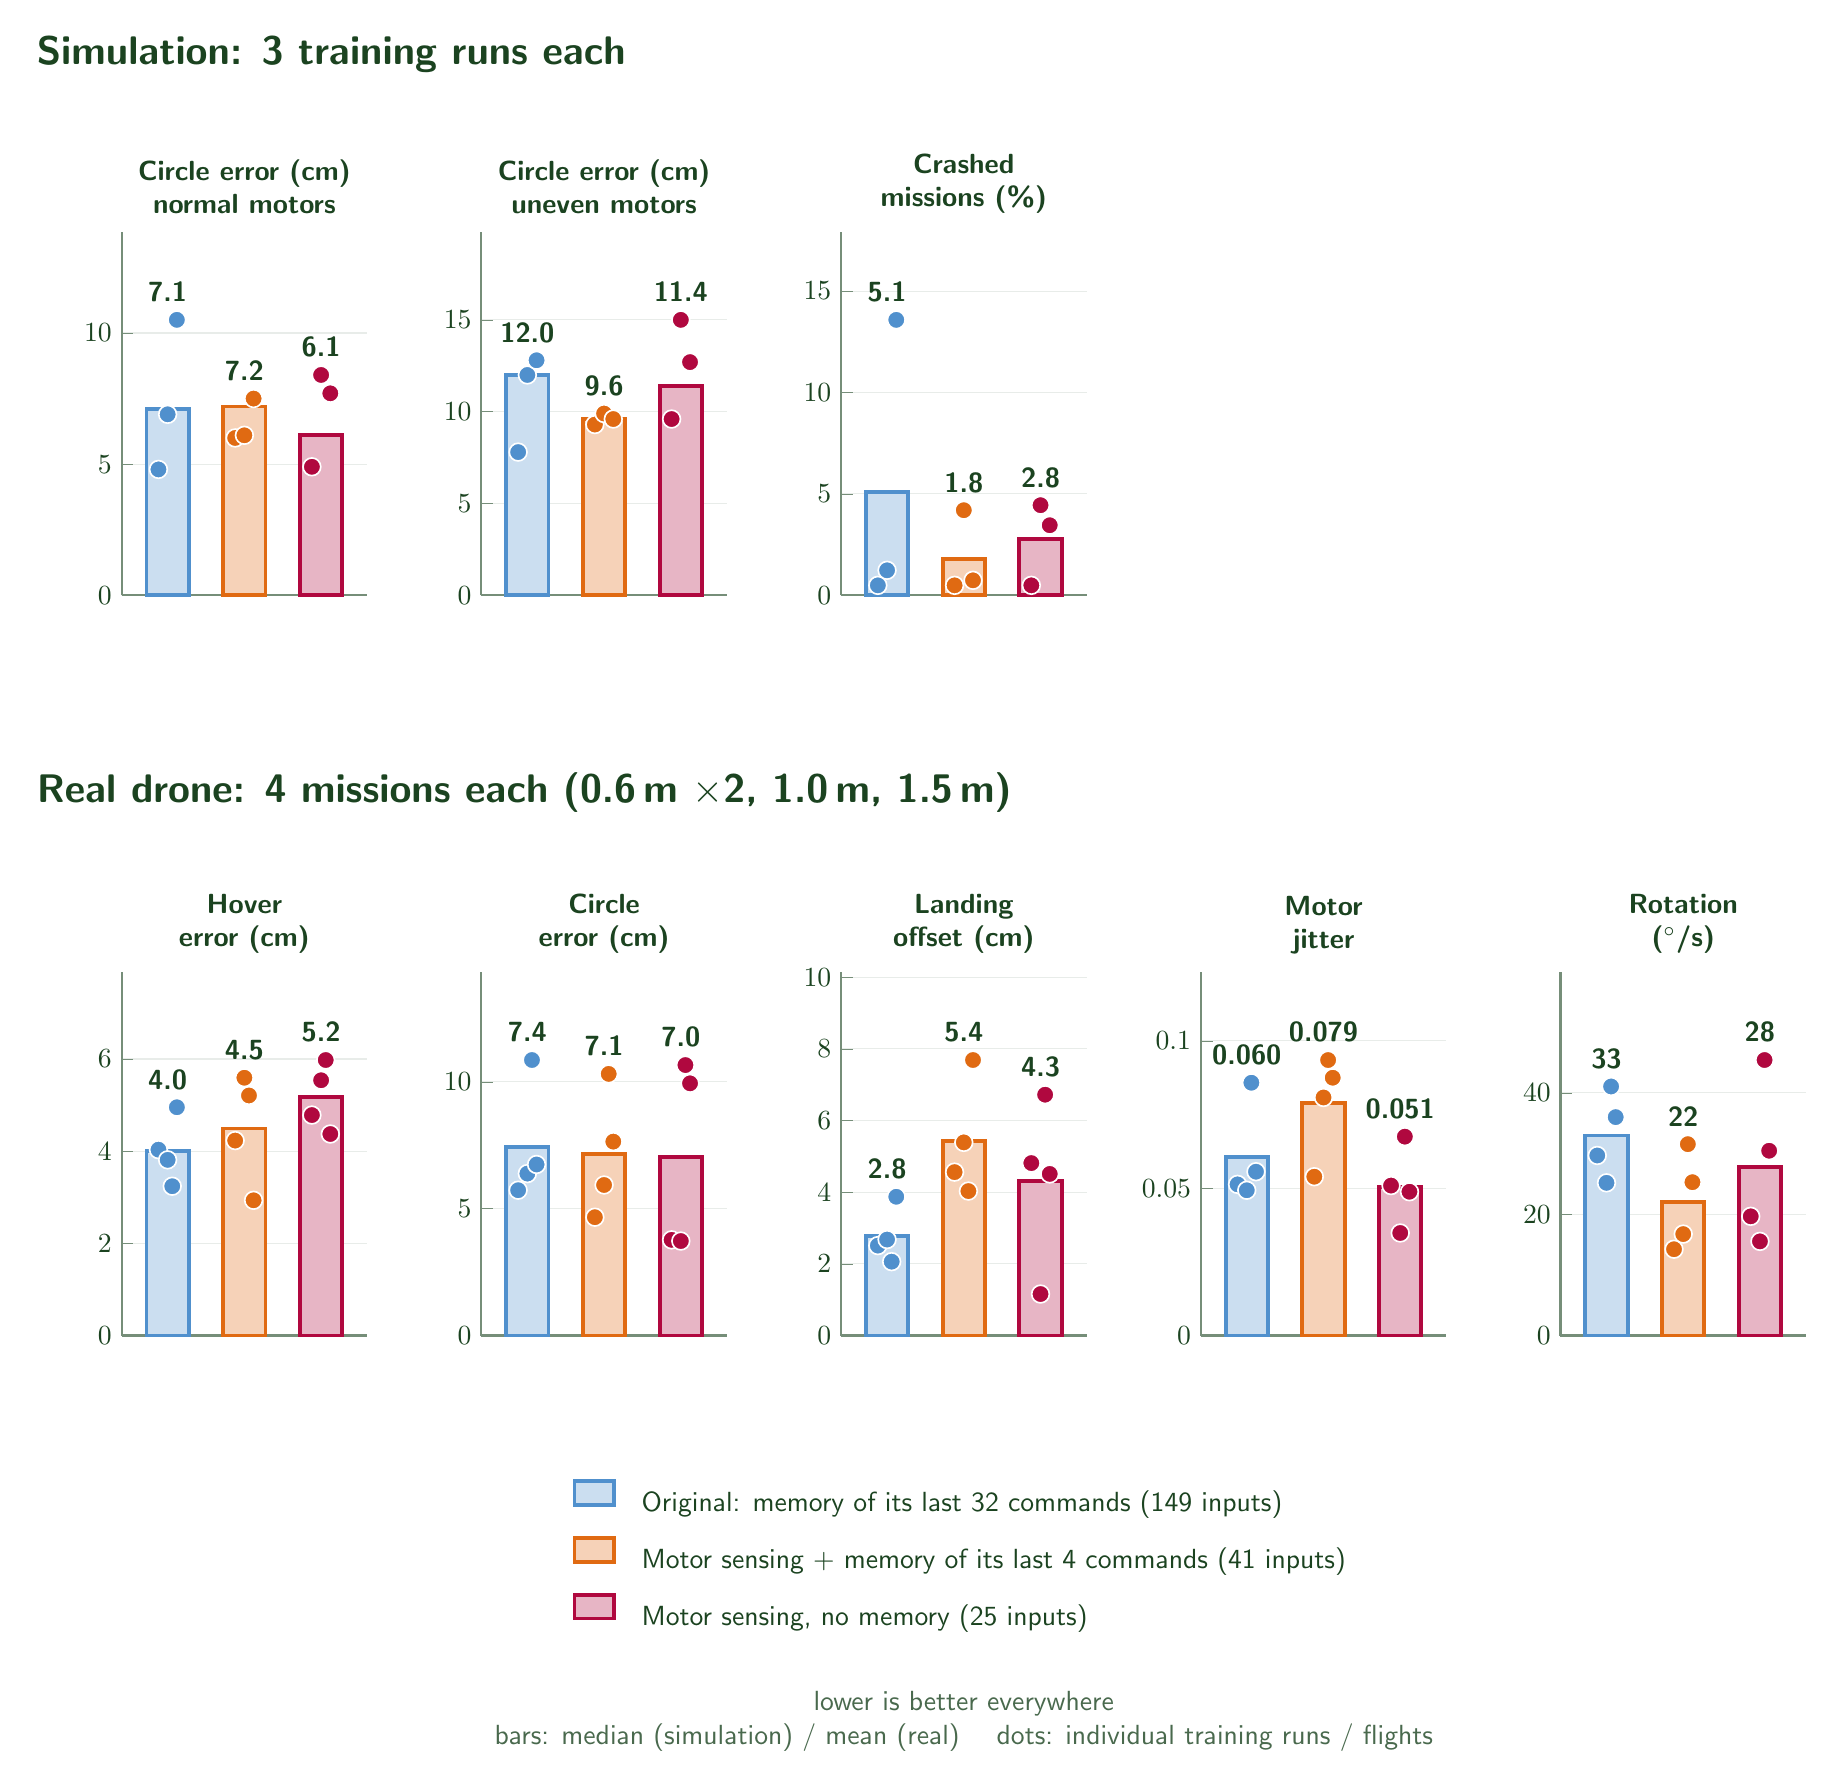
\begin{tikzpicture}
  \begin{groupplot}[group style={group name=sim, group size=3 by 1, horizontal sep=1.45cm},
    width=5.6cm, height=6.2cm, axis x line*=bottom, axis y line*=left,
    axis line style={ink!60, line width=0.8pt}, tick style={ink!60},
    ymajorgrids, grid style={ink!10}, tick label style={font=\normalsize, text=ink},
    xticklabel style={align=center, font=\normalsize\bfseries},
    title style={align=center, font=\normalsize\bfseries, text=ink, yshift=-3pt},
    scaled y ticks=false, clip=false, enlarge x limits=false,
      width=4.7cm]
\nextgroupplot[title={Circle error (cm)\\normal motors}, xmin=-0.6, xmax=2.6, ymin=0, ymax=13.860000000000001, xtick=\empty]
\addplot[ybar, bar width=0.55, fill=cI!30, draw=cI, line width=1.4pt] coordinates {(0,7.1000)};
\addplot[only marks, mark=*, mark size=3.2pt, color=cI, mark options={draw=white, line width=0.6pt}] coordinates {(-0.12,4.8000) (0.00,6.9000) (0.12,10.5000)};
\node[anchor=south, font=\normalsize\bfseries, text=ink] at (axis cs:0,10.5000) [yshift=3pt] {7.1};
\addplot[ybar, bar width=0.55, fill=cC!30, draw=cC, line width=1.4pt] coordinates {(1,7.2000)};
\addplot[only marks, mark=*, mark size=3.2pt, color=cC, mark options={draw=white, line width=0.6pt}] coordinates {(0.88,6.0000) (1.00,6.1000) (1.12,7.5000)};
\node[anchor=south, font=\normalsize\bfseries, text=ink] at (axis cs:1,7.5000) [yshift=3pt] {7.2};
\addplot[ybar, bar width=0.55, fill=cE!30, draw=cE, line width=1.4pt] coordinates {(2,6.1000)};
\addplot[only marks, mark=*, mark size=3.2pt, color=cE, mark options={draw=white, line width=0.6pt}] coordinates {(1.88,4.9000) (2.00,8.4000) (2.12,7.7000)};
\node[anchor=south, font=\normalsize\bfseries, text=ink] at (axis cs:2,8.4000) [yshift=3pt] {6.1};
\nextgroupplot[title={Circle error (cm)\\uneven motors}, xmin=-0.6, xmax=2.6, ymin=0, ymax=19.8, xtick=\empty]
\addplot[ybar, bar width=0.55, fill=cI!30, draw=cI, line width=1.4pt] coordinates {(0,12.0000)};
\addplot[only marks, mark=*, mark size=3.2pt, color=cI, mark options={draw=white, line width=0.6pt}] coordinates {(-0.12,7.8000) (0.00,12.0000) (0.12,12.8000)};
\node[anchor=south, font=\normalsize\bfseries, text=ink] at (axis cs:0,12.8000) [yshift=3pt] {12.0};
\addplot[ybar, bar width=0.55, fill=cC!30, draw=cC, line width=1.4pt] coordinates {(1,9.6000)};
\addplot[only marks, mark=*, mark size=3.2pt, color=cC, mark options={draw=white, line width=0.6pt}] coordinates {(0.88,9.3000) (1.00,9.9000) (1.12,9.6000)};
\node[anchor=south, font=\normalsize\bfseries, text=ink] at (axis cs:1,9.9000) [yshift=3pt] {9.6};
\addplot[ybar, bar width=0.55, fill=cE!30, draw=cE, line width=1.4pt] coordinates {(2,11.4000)};
\addplot[only marks, mark=*, mark size=3.2pt, color=cE, mark options={draw=white, line width=0.6pt}] coordinates {(1.88,9.6000) (2.00,15.0000) (2.12,12.7000)};
\node[anchor=south, font=\normalsize\bfseries, text=ink] at (axis cs:2,15.0000) [yshift=3pt] {11.4};
\nextgroupplot[title={Crashed\\missions (\%)}, xmin=-0.6, xmax=2.6, ymin=0, ymax=17.925925925925927, xtick=\empty]
\addplot[ybar, bar width=0.55, fill=cI!30, draw=cI, line width=1.4pt] coordinates {(0,5.1029)};
\addplot[only marks, mark=*, mark size=3.2pt, color=cI, mark options={draw=white, line width=0.6pt}] coordinates {(-0.12,0.4938) (0.00,1.2346) (0.12,13.5802)};
\node[anchor=south, font=\normalsize\bfseries, text=ink] at (axis cs:0,13.5802) [yshift=3pt] {5.1};
\addplot[ybar, bar width=0.55, fill=cC!30, draw=cC, line width=1.4pt] coordinates {(1,1.8107)};
\addplot[only marks, mark=*, mark size=3.2pt, color=cC, mark options={draw=white, line width=0.6pt}] coordinates {(0.88,0.4938) (1.00,4.1975) (1.12,0.7407)};
\node[anchor=south, font=\normalsize\bfseries, text=ink] at (axis cs:1,4.1975) [yshift=3pt] {1.8};
\addplot[ybar, bar width=0.55, fill=cE!30, draw=cE, line width=1.4pt] coordinates {(2,2.7984)};
\addplot[only marks, mark=*, mark size=3.2pt, color=cE, mark options={draw=white, line width=0.6pt}] coordinates {(1.88,0.4938) (2.00,4.4444) (2.12,3.4568)};
\node[anchor=south, font=\normalsize\bfseries, text=ink] at (axis cs:2,4.4444) [yshift=3pt] {2.8};
  \end{groupplot}
  \node[anchor=south west, font=\Large\bfseries, text=ink] at ($(sim c1r1.north west)+(-1.2,1.9)$)
       {Simulation: 3 training runs each};

  \begin{scope}[yshift=-9.4cm]
  \begin{groupplot}[group style={group name=real, group size=5 by 1, horizontal sep=1.45cm},
    width=5.6cm, height=6.2cm, axis x line*=bottom, axis y line*=left,
    axis line style={ink!60, line width=0.8pt}, tick style={ink!60},
    ymajorgrids, grid style={ink!10}, tick label style={font=\normalsize, text=ink},
    xticklabel style={align=center, font=\normalsize\bfseries},
    title style={align=center, font=\normalsize\bfseries, text=ink, yshift=-3pt},
    scaled y ticks=false, clip=false, enlarge x limits=false,
      width=4.7cm]
\nextgroupplot[title={Hover\\error (cm)}, xmin=-0.6, xmax=2.6, ymin=0, ymax=7.890086073971017, xtick=\empty]
\addplot[ybar, bar width=0.55, fill=cI!30, draw=cI, line width=1.4pt] coordinates {(0,4.0087)};
\addplot[only marks, mark=*, mark size=3.2pt, color=cI, mark options={draw=white, line width=0.6pt}] coordinates {(-0.12,4.0324) (0.00,3.8109) (0.12,4.9522) (0.06,3.2393)};
\node[anchor=south, font=\normalsize\bfseries, text=ink] at (axis cs:0,4.9522) [yshift=3pt] {4.0};
\addplot[ybar, bar width=0.55, fill=cC!30, draw=cC, line width=1.4pt] coordinates {(1,4.4910)};
\addplot[only marks, mark=*, mark size=3.2pt, color=cC, mark options={draw=white, line width=0.6pt}] coordinates {(0.88,4.2294) (1.00,5.5928) (1.12,2.9338) (1.06,5.2080)};
\node[anchor=south, font=\normalsize\bfseries, text=ink] at (axis cs:1,5.5928) [yshift=3pt] {4.5};
\addplot[ybar, bar width=0.55, fill=cE!30, draw=cE, line width=1.4pt] coordinates {(2,5.1677)};
\addplot[only marks, mark=*, mark size=3.2pt, color=cE, mark options={draw=white, line width=0.6pt}] coordinates {(1.88,4.7829) (2.00,5.5383) (2.12,4.3722) (2.06,5.9773)};
\node[anchor=south, font=\normalsize\bfseries, text=ink] at (axis cs:2,5.9773) [yshift=3pt] {5.2};
\nextgroupplot[title={Circle\\error (cm)}, xmin=-0.6, xmax=2.6, ymin=0, ymax=14.334500411604683, xtick=\empty]
\addplot[ybar, bar width=0.55, fill=cI!30, draw=cI, line width=1.4pt] coordinates {(0,7.4279)};
\addplot[only marks, mark=*, mark size=3.2pt, color=cI, mark options={draw=white, line width=0.6pt}] coordinates {(-0.12,5.7279) (0.00,6.3828) (0.12,6.7416) (0.06,10.8595)};
\node[anchor=south, font=\normalsize\bfseries, text=ink] at (axis cs:0,10.8595) [yshift=3pt] {7.4};
\addplot[ybar, bar width=0.55, fill=cC!30, draw=cC, line width=1.4pt] coordinates {(1,7.1380)};
\addplot[only marks, mark=*, mark size=3.2pt, color=cC, mark options={draw=white, line width=0.6pt}] coordinates {(0.88,4.6633) (1.00,5.9336) (1.12,7.6430) (1.06,10.3119)};
\node[anchor=south, font=\normalsize\bfseries, text=ink] at (axis cs:1,10.3119) [yshift=3pt] {7.1};
\addplot[ybar, bar width=0.55, fill=cE!30, draw=cE, line width=1.4pt] coordinates {(2,7.0236)};
\addplot[only marks, mark=*, mark size=3.2pt, color=cE, mark options={draw=white, line width=0.6pt}] coordinates {(1.88,3.7703) (2.00,3.7240) (2.12,9.9399) (2.06,10.6603)};
\node[anchor=south, font=\normalsize\bfseries, text=ink] at (axis cs:2,10.6603) [yshift=3pt] {7.0};
\nextgroupplot[title={Landing\\offset (cm)}, xmin=-0.6, xmax=2.6, ymin=0, ymax=10.147382262306337, xtick=\empty]
\addplot[ybar, bar width=0.55, fill=cI!30, draw=cI, line width=1.4pt] coordinates {(0,2.7799)};
\addplot[only marks, mark=*, mark size=3.2pt, color=cI, mark options={draw=white, line width=0.6pt}] coordinates {(-0.12,2.5091) (0.00,2.6778) (0.12,3.8716) (0.06,2.0610)};
\node[anchor=south, font=\normalsize\bfseries, text=ink] at (axis cs:0,3.8716) [yshift=3pt] {2.8};
\addplot[ybar, bar width=0.55, fill=cC!30, draw=cC, line width=1.4pt] coordinates {(1,5.4165)};
\addplot[only marks, mark=*, mark size=3.2pt, color=cC, mark options={draw=white, line width=0.6pt}] coordinates {(0.88,4.5592) (1.00,5.3891) (1.12,7.6874) (1.06,4.0304)};
\node[anchor=south, font=\normalsize\bfseries, text=ink] at (axis cs:1,7.6874) [yshift=3pt] {5.4};
\addplot[ybar, bar width=0.55, fill=cE!30, draw=cE, line width=1.4pt] coordinates {(2,4.2994)};
\addplot[only marks, mark=*, mark size=3.2pt, color=cE, mark options={draw=white, line width=0.6pt}] coordinates {(1.88,4.8115) (2.00,1.1574) (2.12,4.5087) (2.06,6.7198)};
\node[anchor=south, font=\normalsize\bfseries, text=ink] at (axis cs:2,6.7198) [yshift=3pt] {4.3};
\nextgroupplot[title={Motor\\jitter}, xmin=-0.6, xmax=2.6, ymin=0, ymax=0.12343402122908388, xtick=\empty, yticklabel style={/pgf/number format/fixed, /pgf/number format/precision=2}]
\addplot[ybar, bar width=0.55, fill=cI!30, draw=cI, line width=1.4pt] coordinates {(0,0.0605)};
\addplot[only marks, mark=*, mark size=3.2pt, color=cI, mark options={draw=white, line width=0.6pt}] coordinates {(-0.12,0.0513) (0.00,0.0493) (0.12,0.0556) (0.06,0.0858)};
\node[anchor=south, font=\normalsize\bfseries, text=ink] at (axis cs:0,0.0858) [yshift=3pt] {0.060};
\addplot[ybar, bar width=0.55, fill=cC!30, draw=cC, line width=1.4pt] coordinates {(1,0.0789)};
\addplot[only marks, mark=*, mark size=3.2pt, color=cC, mark options={draw=white, line width=0.6pt}] coordinates {(0.88,0.0539) (1.00,0.0808) (1.12,0.0875) (1.06,0.0935)};
\node[anchor=south, font=\normalsize\bfseries, text=ink] at (axis cs:1,0.0935) [yshift=3pt] {0.079};
\addplot[ybar, bar width=0.55, fill=cE!30, draw=cE, line width=1.4pt] coordinates {(2,0.0505)};
\addplot[only marks, mark=*, mark size=3.2pt, color=cE, mark options={draw=white, line width=0.6pt}] coordinates {(1.88,0.0509) (2.00,0.0348) (2.12,0.0488) (2.06,0.0675)};
\node[anchor=south, font=\normalsize\bfseries, text=ink] at (axis cs:2,0.0675) [yshift=3pt] {0.051};
\nextgroupplot[title={Rotation\\($^\circ$/s)}, xmin=-0.6, xmax=2.6, ymin=0, ymax=59.95589788452559, xtick=\empty]
\addplot[ybar, bar width=0.55, fill=cI!30, draw=cI, line width=1.4pt] coordinates {(0,32.9799)};
\addplot[only marks, mark=*, mark size=3.2pt, color=cI, mark options={draw=white, line width=0.6pt}] coordinates {(-0.12,29.6817) (0.00,25.1704) (0.12,36.0089) (0.06,41.0585)};
\node[anchor=south, font=\normalsize\bfseries, text=ink] at (axis cs:0,41.0585) [yshift=3pt] {33};
\addplot[ybar, bar width=0.55, fill=cC!30, draw=cC, line width=1.4pt] coordinates {(1,21.9437)};
\addplot[only marks, mark=*, mark size=3.2pt, color=cC, mark options={draw=white, line width=0.6pt}] coordinates {(0.88,14.2267) (1.00,16.7217) (1.12,25.2801) (1.06,31.5464)};
\node[anchor=south, font=\normalsize\bfseries, text=ink] at (axis cs:1,31.5464) [yshift=3pt] {22};
\addplot[ybar, bar width=0.55, fill=cE!30, draw=cE, line width=1.4pt] coordinates {(2,27.7644)};
\addplot[only marks, mark=*, mark size=3.2pt, color=cE, mark options={draw=white, line width=0.6pt}] coordinates {(1.88,19.6502) (2.00,15.5230) (2.12,30.4630) (2.06,45.4211)};
\node[anchor=south, font=\normalsize\bfseries, text=ink] at (axis cs:2,45.4211) [yshift=3pt] {28};
  \end{groupplot}
  \end{scope}
  \node[anchor=south west, font=\Large\bfseries, text=ink] at ($(real c1r1.north west)+(-1.2,1.9)$)
       {Real drone: 4 missions each (0.6\,m $\times$2, 1.0\,m, 1.5\,m)};

  % key
  \matrix[anchor=north, column sep=6pt, row sep=3pt, font=\normalsize, text=ink]
      at ($(real c3r1.south)+(0,-1.7)$) {
    \fill[cI!30] (0,0) rectangle (0.5,0.3); \draw[cI, line width=1.4pt] (0,0) rectangle (0.5,0.3); &
      \node[anchor=west]{Original: memory of its last 32 commands (149 inputs)}; \\
    \fill[cC!30] (0,0) rectangle (0.5,0.3); \draw[cC, line width=1.4pt] (0,0) rectangle (0.5,0.3); &
      \node[anchor=west]{Motor sensing + memory of its last 4 commands (41 inputs)}; \\
    \fill[cE!30] (0,0) rectangle (0.5,0.3); \draw[cE, line width=1.4pt] (0,0) rectangle (0.5,0.3); &
      \node[anchor=west]{Motor sensing, no memory (25 inputs)}; \\
  };
  \node[anchor=north, align=center, font=\normalsize, text=ink!80] at ($(real c3r1.south)+(0,-4.4)$)
       {lower is better everywhere\\
        bars: median (simulation) / mean (real) \quad dots: individual training runs / flights};
\end{tikzpicture}
\end{document}
